% ============================================================================
% Backtesting framework and methodology
% ============================================================================
\section{Backtesting framework and methodology}
\label{sec:framework}

We evaluate strategies through a daily simulation that updates model
estimates from the available history, constructs portfolios, and measures
their subsequent returns. By separating these tasks within a common
framework, we can compare trading rules and model settings while keeping
the data flow and portfolio accounting consistent.

\subsection{Framework structure}

The framework separates three tasks:
\begin{itemize}
    \item \textbf{Models.} Convert return history into estimates and signals.
    \item \textbf{Strategies.} Use model outputs to choose portfolio weights.
    \item \textbf{Simulator.} Track positions, trades, fees, and portfolio value.
\end{itemize}
The daily return history first enters the PCA model, whose components
and volatility estimates feed the factor regression. The regression then
produces stock alphas, exposures, and residuals, which strategies can use
directly or pass to additional signal models.
Models run in dependency order so that each receives the estimates it
requires before producing its own output.

Each strategy receives the model outputs and its current portfolio
weights, then returns target weights for the simulator to implement.
The simulator calculates the required trades and fees, applies the next
day's returns to the resulting positions, and passes the updated weights
back to the strategy. Keeping this accounting separate from the trading
rule allows several strategies to share model estimates while maintaining
independent portfolios, reducing repeated computation and ensuring that
their decisions use comparable inputs.

\begin{figure}[htbp]
    \centering
    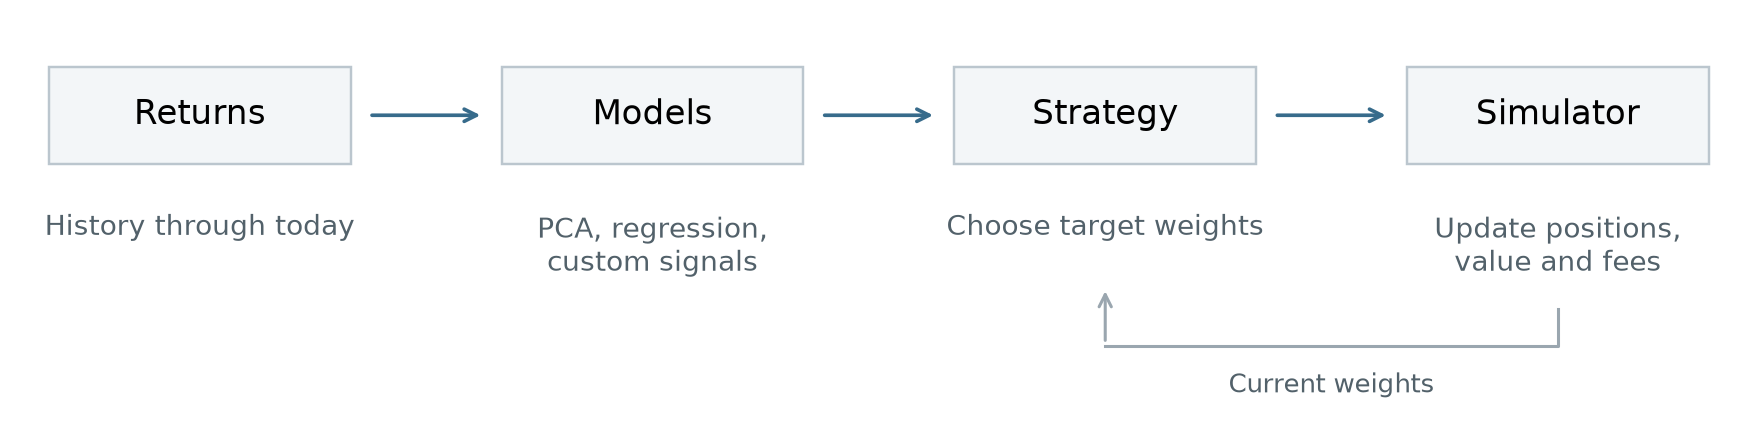
\includegraphics[width=\linewidth]{figures/framework_components.png}
    \caption{Daily data flow through the backtesting framework. Return
    history available through the current close enters the model sequence,
    which includes PCA, factor regression, and any custom signals.
    The strategy converts these outputs into target portfolio weights,
    while the simulator handles positions, returns, trades, and fees.
    The return arrow supplies the strategy with current weights after
    market movements, allowing it to calculate the next adjustment.
    The diagram shows one strategy, but several independent portfolios
    can use the same model outputs.}
    \label{fig:framework-components}
\end{figure}

\subsection{Rolling estimates}

Our PCA and factor models use rolling windows: fixed-length segments of
recent return history that advance as new observations arrive. Each model
has a configurable window length and refitting interval, which determine
how much history enters a fit and how often the estimate changes.
For example, a PCA model with a 500-day window and a five-day interval
fits on the latest 500 returns, reuses the estimate for four more days,
and then refits on the updated window. Because the factor regression has
its own window and interval, a strategy can estimate common factors from
a longer history while allowing stock exposures to respond more quickly
to recent observations.

At a PCA refit, we subtract each stock's mean and divide by its sample
standard deviation within that window, preventing highly volatile stocks
from dominating solely because of their larger return variation. After
retaining the leading \(K\) components, the regression converts them into
factor weights using the same volatility estimates and calculates factor
returns over its own window. Regressing each stock's returns on these
factors and an intercept then produces its estimated alpha and exposures.

To maintain a consistent factor definition within each regression, all
observations use the same active PCA weights. A new PCA estimate therefore
triggers a regression refit even before the regression's usual interval
elapses. Between refits, coefficients remain fixed while factor returns
and residuals update with each day's observations.

The same timing restriction applies to every stage of estimation,
including standardization, so future returns and volatility cannot enter
an earlier fit. Refitting also leaves earlier trading decisions unchanged.
Together, these conventions avoid look-ahead from model estimation,
although they do not eliminate the selection bias associated with
developing strategies through repeated experiments.

Custom signal models use the same daily flow, managing their own windows
and update schedules from the history of earlier outputs. When a model
learns from a five-day return, for example, that observation enters training
only after the full holding period ends. Strategies receive the updated
estimates through a common interface without changes to the simulation.

\begin{figure}[htbp]
    \centering
    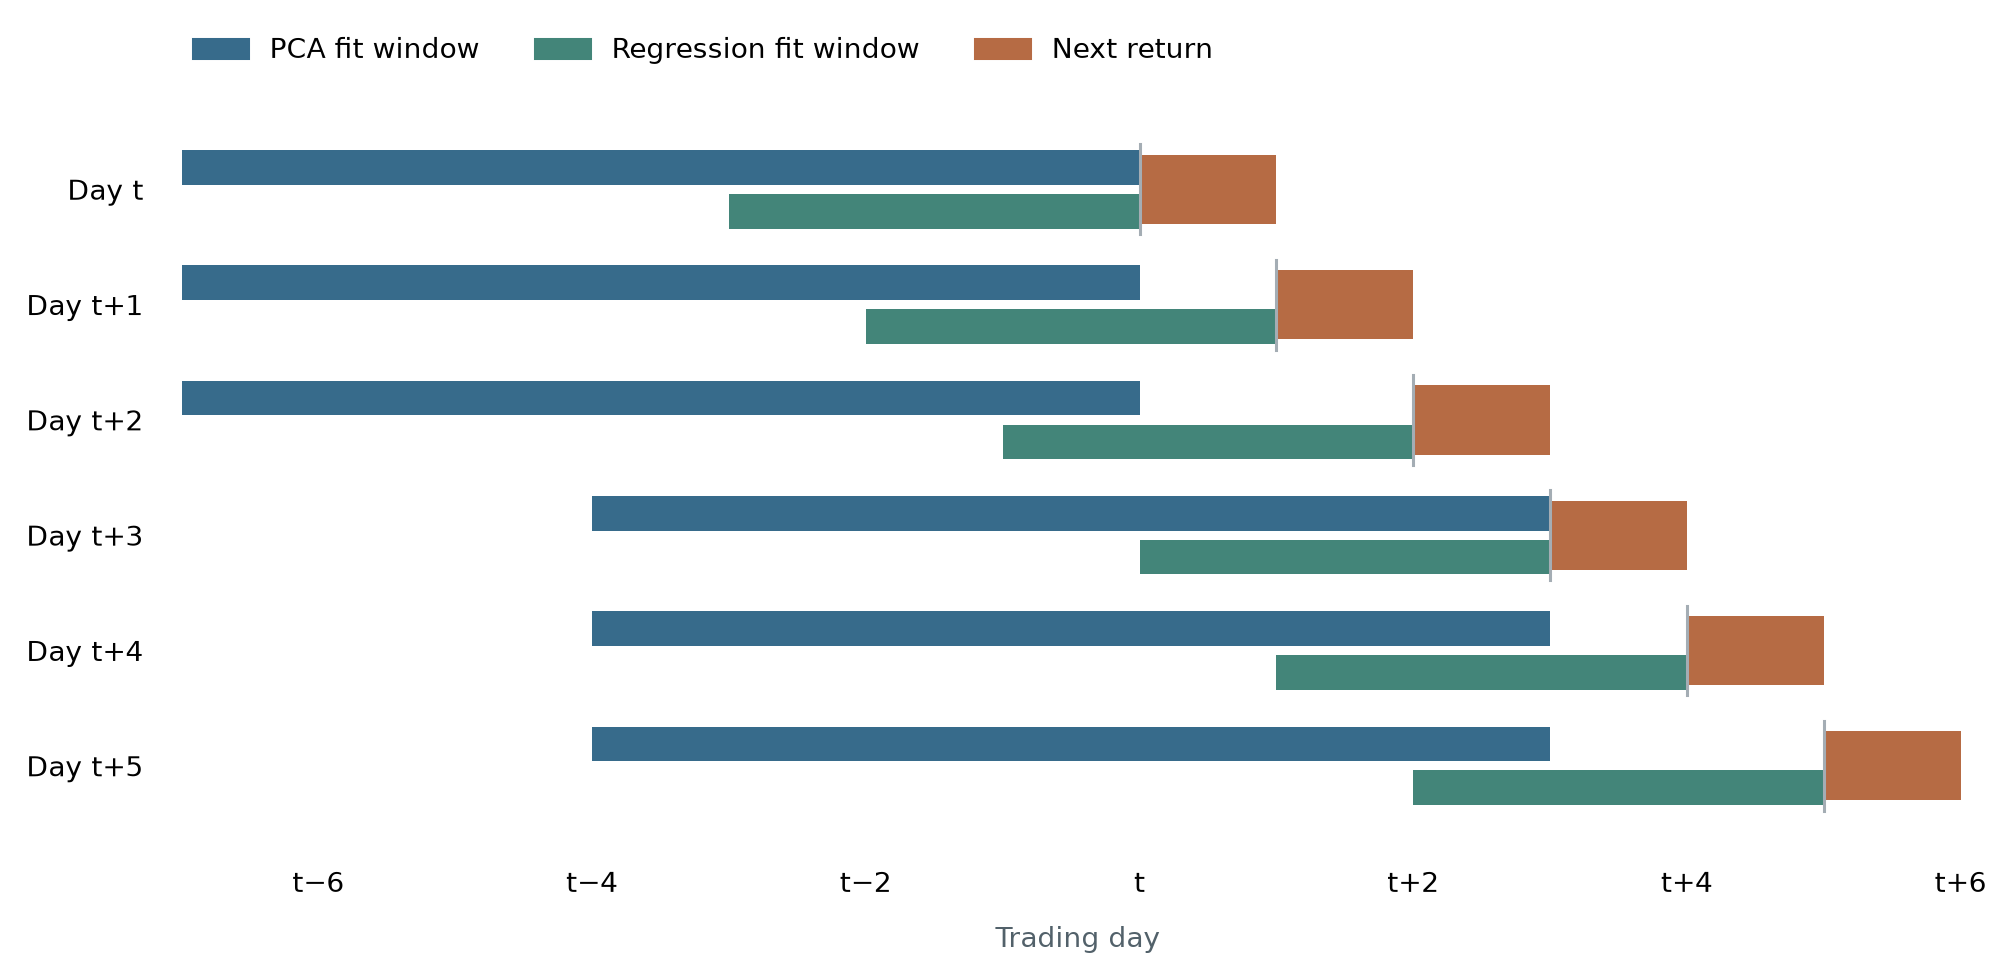
\includegraphics[width=\linewidth]{figures/framework_walkforward.png}
    \caption{Walk-forward estimation over six consecutive decision dates.
    Each row represents the portfolio decision at the indicated day's
    close, marked by the vertical gray line. Blue bars identify the
    observations used by the active PCA estimate, and green bars identify
    the regression window. In this example, PCA refits at \(t\) and
    \(t+3\), so its estimation window remains unchanged for three rows
    before advancing. The regression refits daily using the active PCA
    weights, including a new factor basis when PCA updates. Orange bars
    show the subsequent return interval earned by the chosen portfolio.
    Estimation periods lie entirely before or at the decision close,
    while portfolio returns occur afterward. Window lengths and the
    three-day PCA interval are illustrative rather than strategy defaults.}
    \label{fig:framework-walkforward}
\end{figure}

\subsection{Computational efficiency of PCA}

Rolling PCA requires repeatedly fitting the model as the window advances,
which becomes slow when we test many parameter settings. Our basic
implementation computes all 1,201 eigenvalues and eigenvectors of the
stock covariance matrix, even when we use only five factors. We replace
this full decomposition with an iterative solver that computes only the
largest \(K\) eigenvalues and their eigenvectors. Comparing the methods
on the same return windows, we find that a 500-day fit with 1,201 stocks
and five factors takes about 264 ms with the basic method and 13.1 ms
with the optimized method, giving a median paired speedup of roughly
\(19\times\). The figures below compare runtime across different problem
sizes and show that the resulting eigenvalues and factor subspaces agree
closely. The gain is smaller for small stock universes, but it substantially
reduces the cost of repeated PCA fits on our full dataset.

\begin{figure}[htbp]
    \centering
    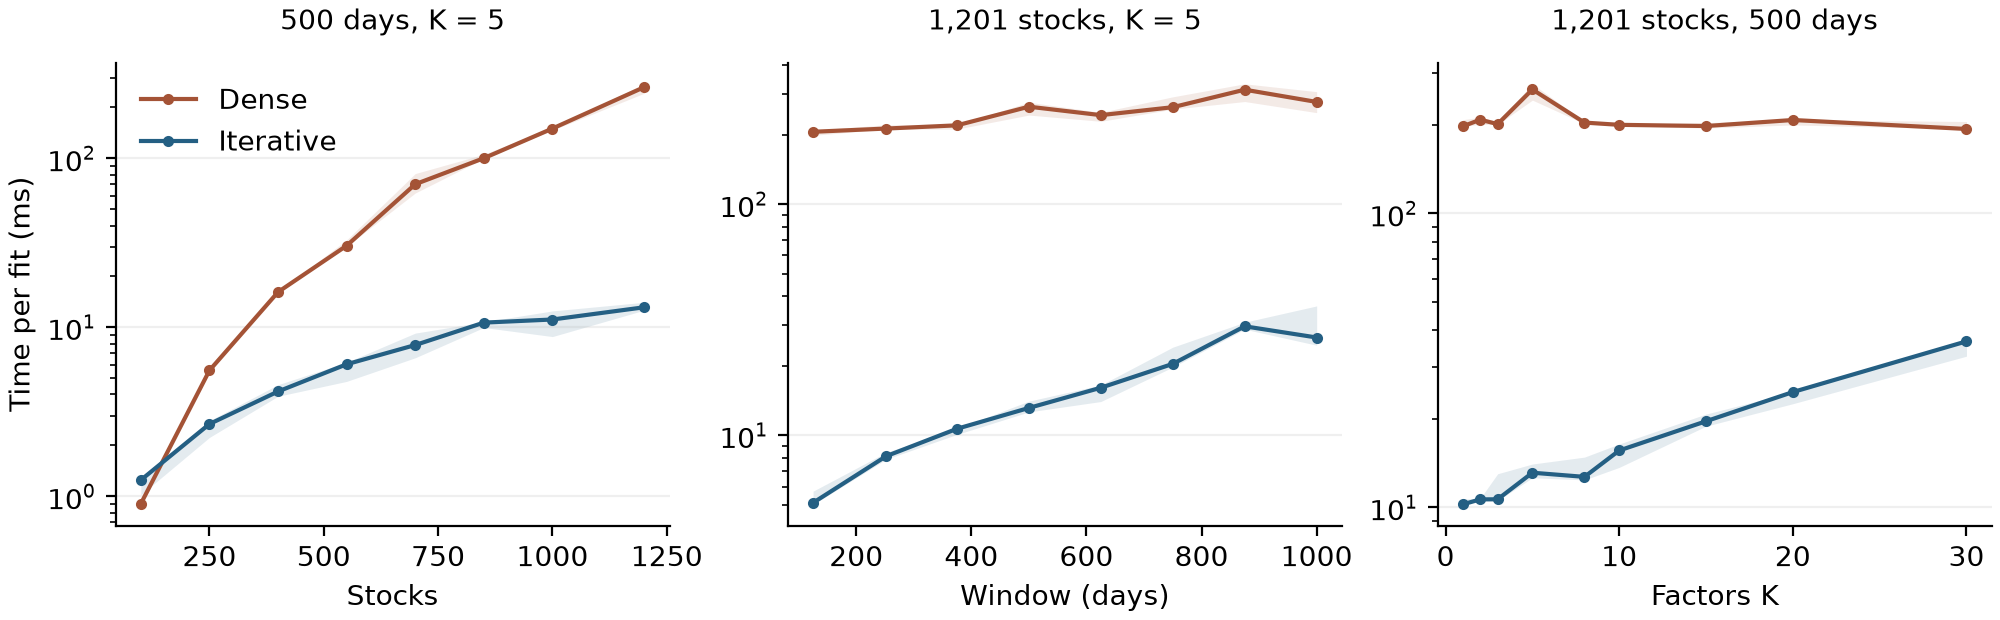
\includegraphics[width=\linewidth]{figures/pca_benchmark.png}
    \caption{PCA runtime as stock count, window length, and factor count
    vary, with other settings fixed as indicated above each panel.
    Points summarize the median of three window medians, each based on
    five runs. Shading spans the window medians rather than a confidence
    interval. Times include standardization and fitting, and the vertical
    axes are logarithmic. The iterative method's
    advantage grows with universe size but decreases as more factors
    are requested.}
    \label{fig:pca-benchmark}
\end{figure}

\begin{figure}[htbp]
    \centering
    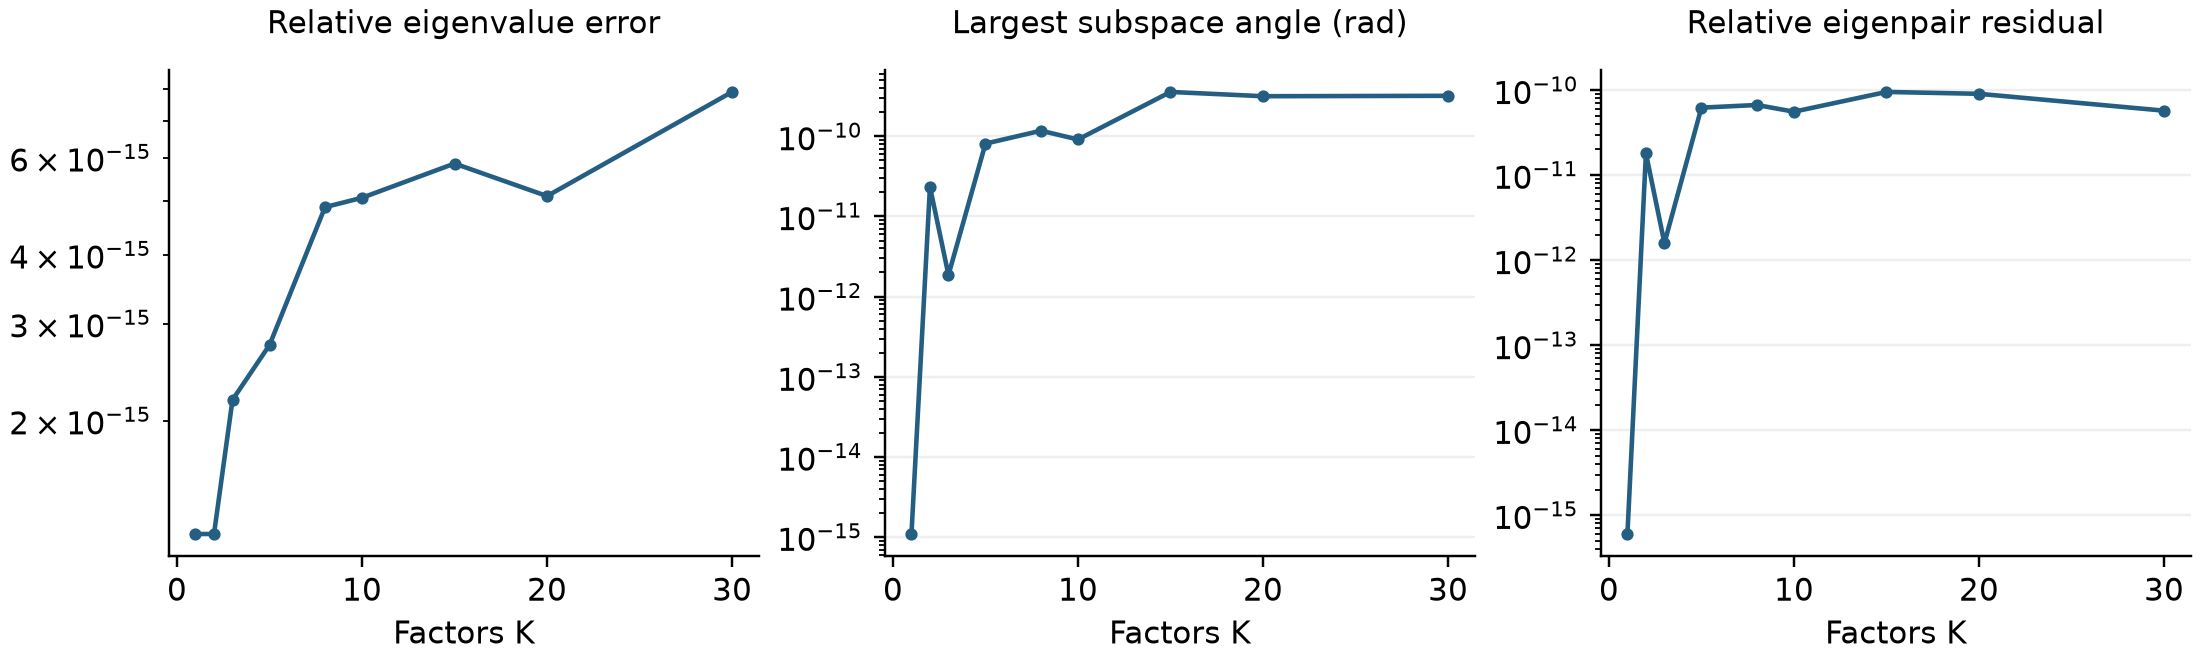
\includegraphics[width=\linewidth]{figures/pca_agreement.png}
    \caption{Numerical accuracy for 1,201 stocks and 500-day windows.
    The panels show relative eigenvalue differences, the largest angle
    between factor subspaces, and relative eigenpair residuals. Subspace
    angles account for arbitrary eigenvector signs, while residuals check
    the covariance eigenvalue equation directly. Each point is the worst
    value across three windows and five fits. Lower is better, and the
    logarithmic vertical axes have different scales. All checks pass
    the respective limits of \(10^{-8}\), \(10^{-6}\) radians, and
    \(10^{-8}\).}
    \label{fig:pca-agreement}
\end{figure}

\subsection{Execution and trading costs}

Our simulator applies daily returns to existing positions before executing
the next portfolio adjustment. Positions carried into day \(t\) therefore
earn that day's returns, while newly chosen weights \(w_{i,t}\) earn
returns on day \(t+1\):
\[
    r_{\mathrm{port},t+1}^{\mathrm{gross}}
    = \sum_i w_{i,t}r_{i,t+1}.
\]
Strategies hold cash until their required estimates are available, after
which we assume execution at the close used to calculate the signal.
This approximates observing prices immediately before the close and
submitting orders in time, but abstracts from processing delays and
differences between observed and executed prices. Introducing an additional
day of delay tests how strongly performance depends on immediate execution.

We calculate turnover from the weights after market movements to the new
targets, capturing the trades needed to restore an allocation even when
its target is unchanged. Positions held without adjustment incur no
rebalancing charge. The baseline deducts 5 basis points per dollar bought
or sold, including both entry and exit, while comparisons at higher fee
levels assess the sensitivity of net returns to execution costs.

\subsection{Strategy development and evaluation}

We divide evaluation into chronological training, validation, and final
holdout periods, using the training sample to develop signals and compare
candidate settings. Validation then assesses their performance on later
observations and informs the final selection. This chronological structure
preserves the order in which information becomes available, whereas a
random split would allow later market conditions to influence choices
evaluated on earlier observations.

Before the final holdout, we fix the trading rules, parameter settings,
cost assumptions, missing-data treatment, and performance measures, then
evaluate the holdout exactly once and retain the result regardless of
performance. This separates the final assessment from strategy selection.
Model estimates continue to update as observations arrive, but their
update rules remain fixed. A 500-day window, for example, continues to
advance without its length being reconsidered in response to holdout
results.

Each strategy section follows the same sequence so readers can compare
the evidence:
\begin{enumerate}
    \item \textbf{Strategy specification.} Explain the signal's motivation
    and conversion into weights, specifying estimation windows, refitting
    and trading intervals, and exposure limits.
    \item \textbf{Performance.} Report gross and net cumulative returns,
    annual results, drawdowns, and turnover to identify concentration in
    exceptional years and the contribution of trading costs.
    \item \textbf{Parameter sensitivity.} Vary nearby settings and factor
    count \(K\) over common dates after the longest warm-up. Compare
    full-sample and rolling estimates to assess how future information
    affects performance and the apparent preferred factor count.
    \item \textbf{Signal validation.} Compare subsequent returns across
    signal-strength groups and holding periods, accounting for dependence
    between overlapping returns when assessing uncertainty.
    \item \textbf{Implementation sensitivity.} Test higher fees, delayed
    execution, and exposure drift to identify dependence on low costs,
    immediate fills, or unintended risk.
    \item \textbf{Final holdout.} Report the fixed strategy's holdout result
    alongside training and validation performance, including deterioration.
\end{enumerate}

We report Sharpe ratios using daily returns, a zero risk-free-rate
convention, and annualization by \(\sqrt{252}\). For the assignment's
information ratio, we subtract fitted market exposure from portfolio
returns, divide their mean by their standard deviation, and apply the
same annualization. We state the benchmark and report market beta so
readers can see whether profits come with market exposure.

\subsection{Limitations}

Our tests address information timing, parameter sensitivity, and execution
assumptions, but the following biases and modeling limits remain relevant
when interpreting performance.

\begin{itemize}
    \item \textbf{Multiple-testing bias and validation overfitting.}
    Searching across signals and settings increases the chance of selecting
    a result that partly reflects luck. Repeated validation also makes
    those observations part of strategy selection, even when individual
    backtests use rolling estimates. Sensitivity checks and a final holdout
    strengthen the evidence without making the selected historical Sharpe
    ratio an unbiased estimate of future performance.

    \item \textbf{Survivorship and universe-selection bias.} The original
    panel contains long histories for 1,201 stocks over 2000--2023 and may
    underrepresent failed firms, delisted securities, and later entrants.
    Its selection procedure is unverified, so we cannot establish that
    the universe matches the securities available on each historical date.
    Rolling estimation restricts the information entering a fit but does
    not correct selection of the stocks themselves.

    \item \textbf{Execution and transaction-cost optimism.} Closing-price
    execution assumes negligible processing time and access to the observed
    price. Proportional fees omit market impact and stock-specific spreads,
    while the baseline also omits borrow costs and availability and assumes
    zero cash interest. These simplifications can overstate implementable
    returns. Higher-fee and delayed-execution tests assess sensitivity but
    do not establish achievable fills at a given portfolio size.

    \item \textbf{Regime dependence and limited external validity.} The
    final holdout covers one subsequent combination of volatility, liquidity,
    and investor behavior. Annual comparisons reveal concentration in
    particular episodes, but a successful holdout does not establish
    performance under different market conditions. Conclusions therefore
    apply to the observed periods without implying stable future returns.
\end{itemize}
